\documentclass[../taasin.tex]{subfiles}
\graphicspath{{\subfix{../figures/}}}
\begin{document}

%%%%%%%%%%%%%%%%%%%%%%%%%%%%%%%%%%%%%%%%%%%%%%%%%%%%%%%%%%%%%%%%%%%%%%

As stated before, our ONV is a vector of dimension 14,400. SNNs, however, expect inputs that vary over time. In addition, the floating point numbers that represent the light intensity at a pixel need to be meaningfully converted into "spikes," or a list of 1's and 0's. This is known as converting data from the "frame" domain to the "spiking" domain, and there are two main conversion schemes that we can use to do this.

In addition to generating spiking inputs, we also introduce a "delta" ONV. Instead of having the eye see light intensities at the current timestep, it sees the difference between the current and previous ONV. In other words, the eye only sees what has changed in the scene, also referred to as "event-based" data. This is shown in figure \ref{fig:three ONVs}. Note that we have positive values if pixels get brighter and negative values if they get darker. This results in sparse input data as the eye doesn't have to keep processing what it has already seen. The delta ONV is more biologically accurate as Ganglion cells in the retina emit spikes only when there is change in the field of view \cite{eventRetina}.

\begin{figure}
    \centering
    \begin{subfigure}[b]{0.45\textwidth}
        \centering
        % \includesvg{onv_normal_prev.svg}
        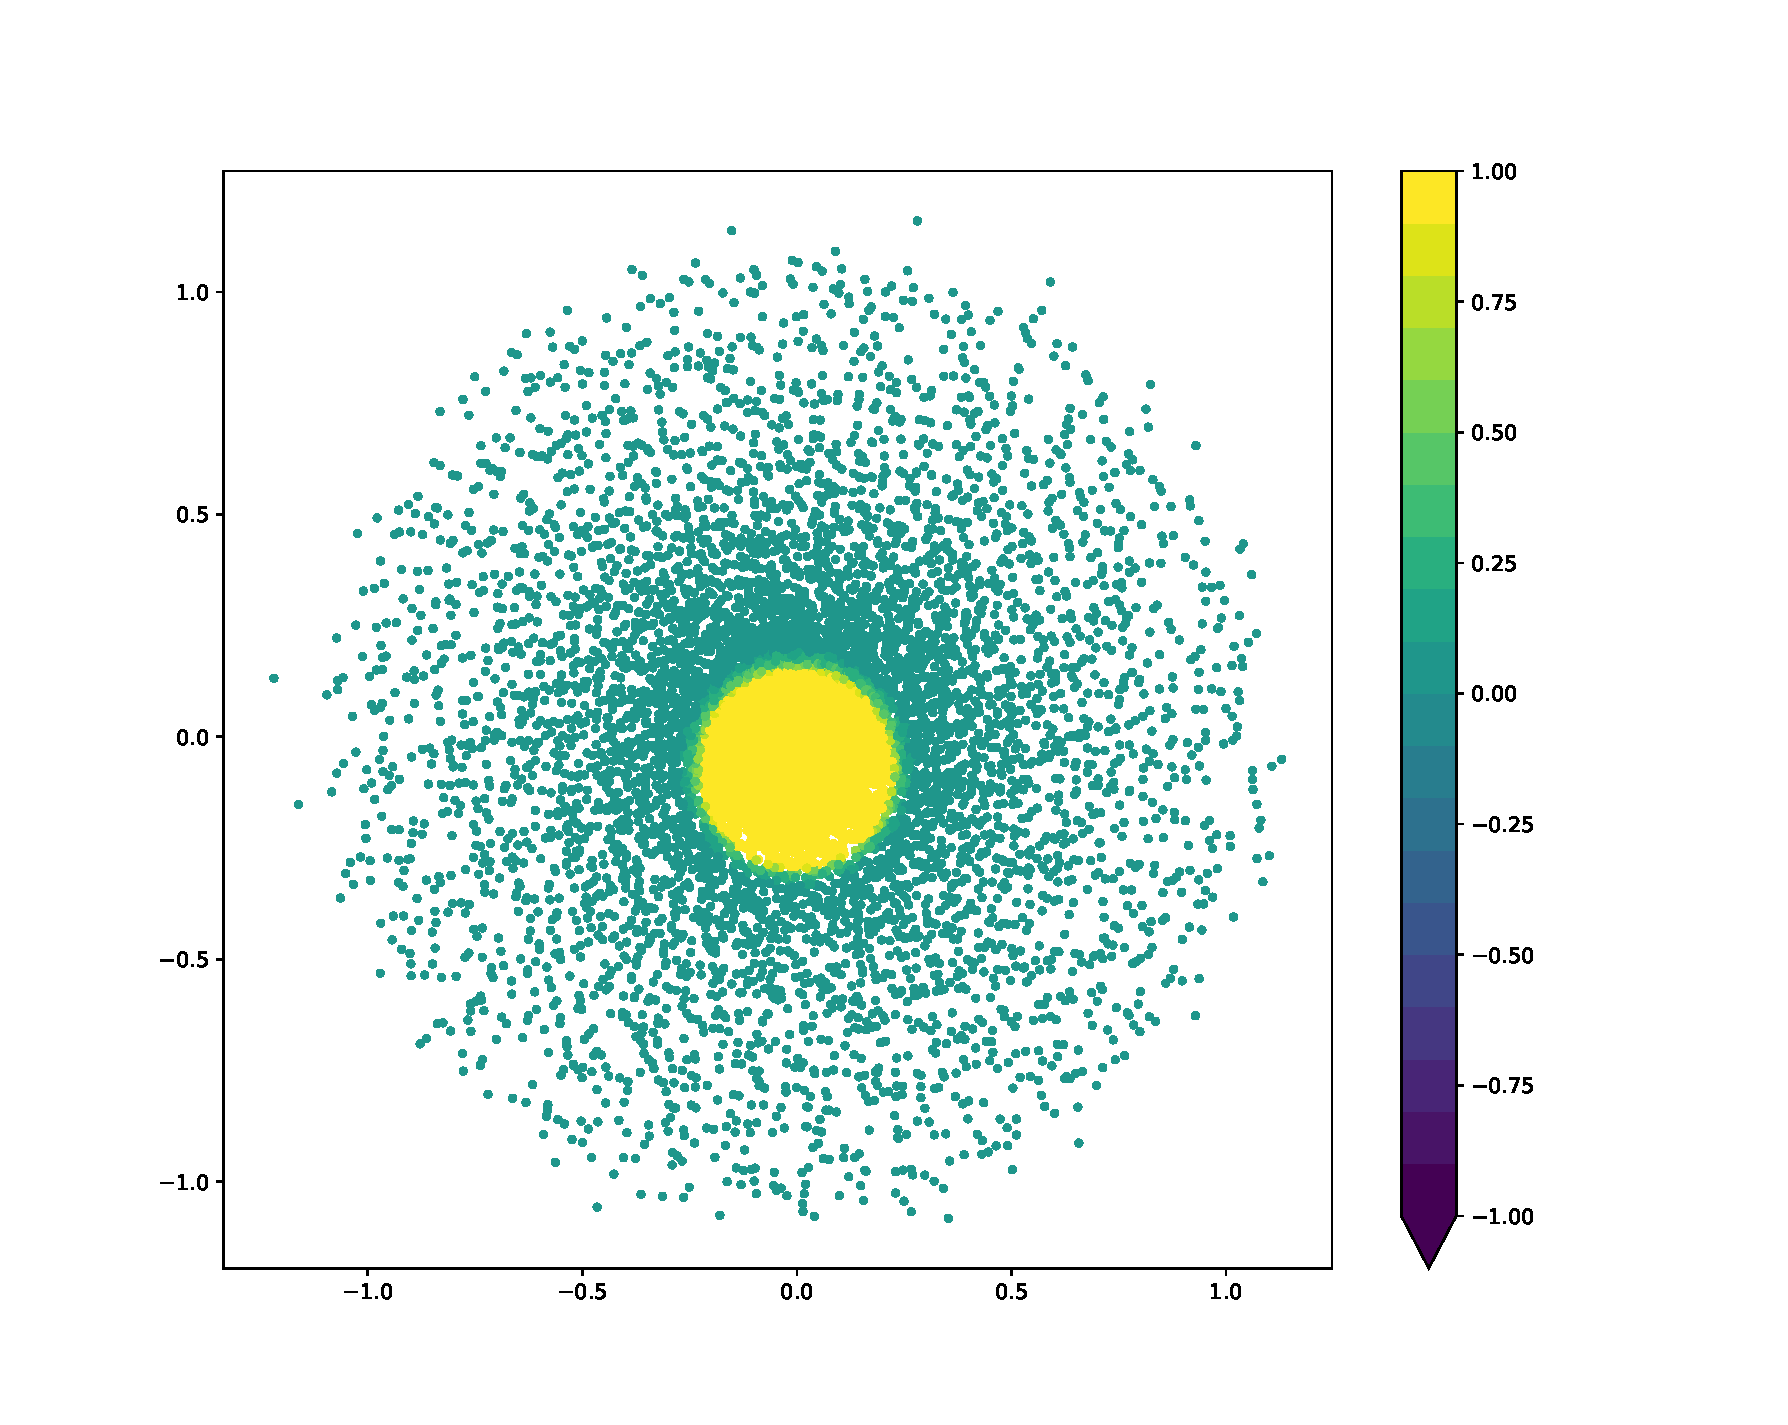
\includegraphics[width=\textwidth]{figures/onv_normal_prev.pdf}
        \caption{Previous ONV}
        \label{fig:onv_prev}
    \end{subfigure}
    \hfill
    \begin{subfigure}[b]{0.45\textwidth}
        \centering
        % \includesvg{onv_normal_cur.svg}
        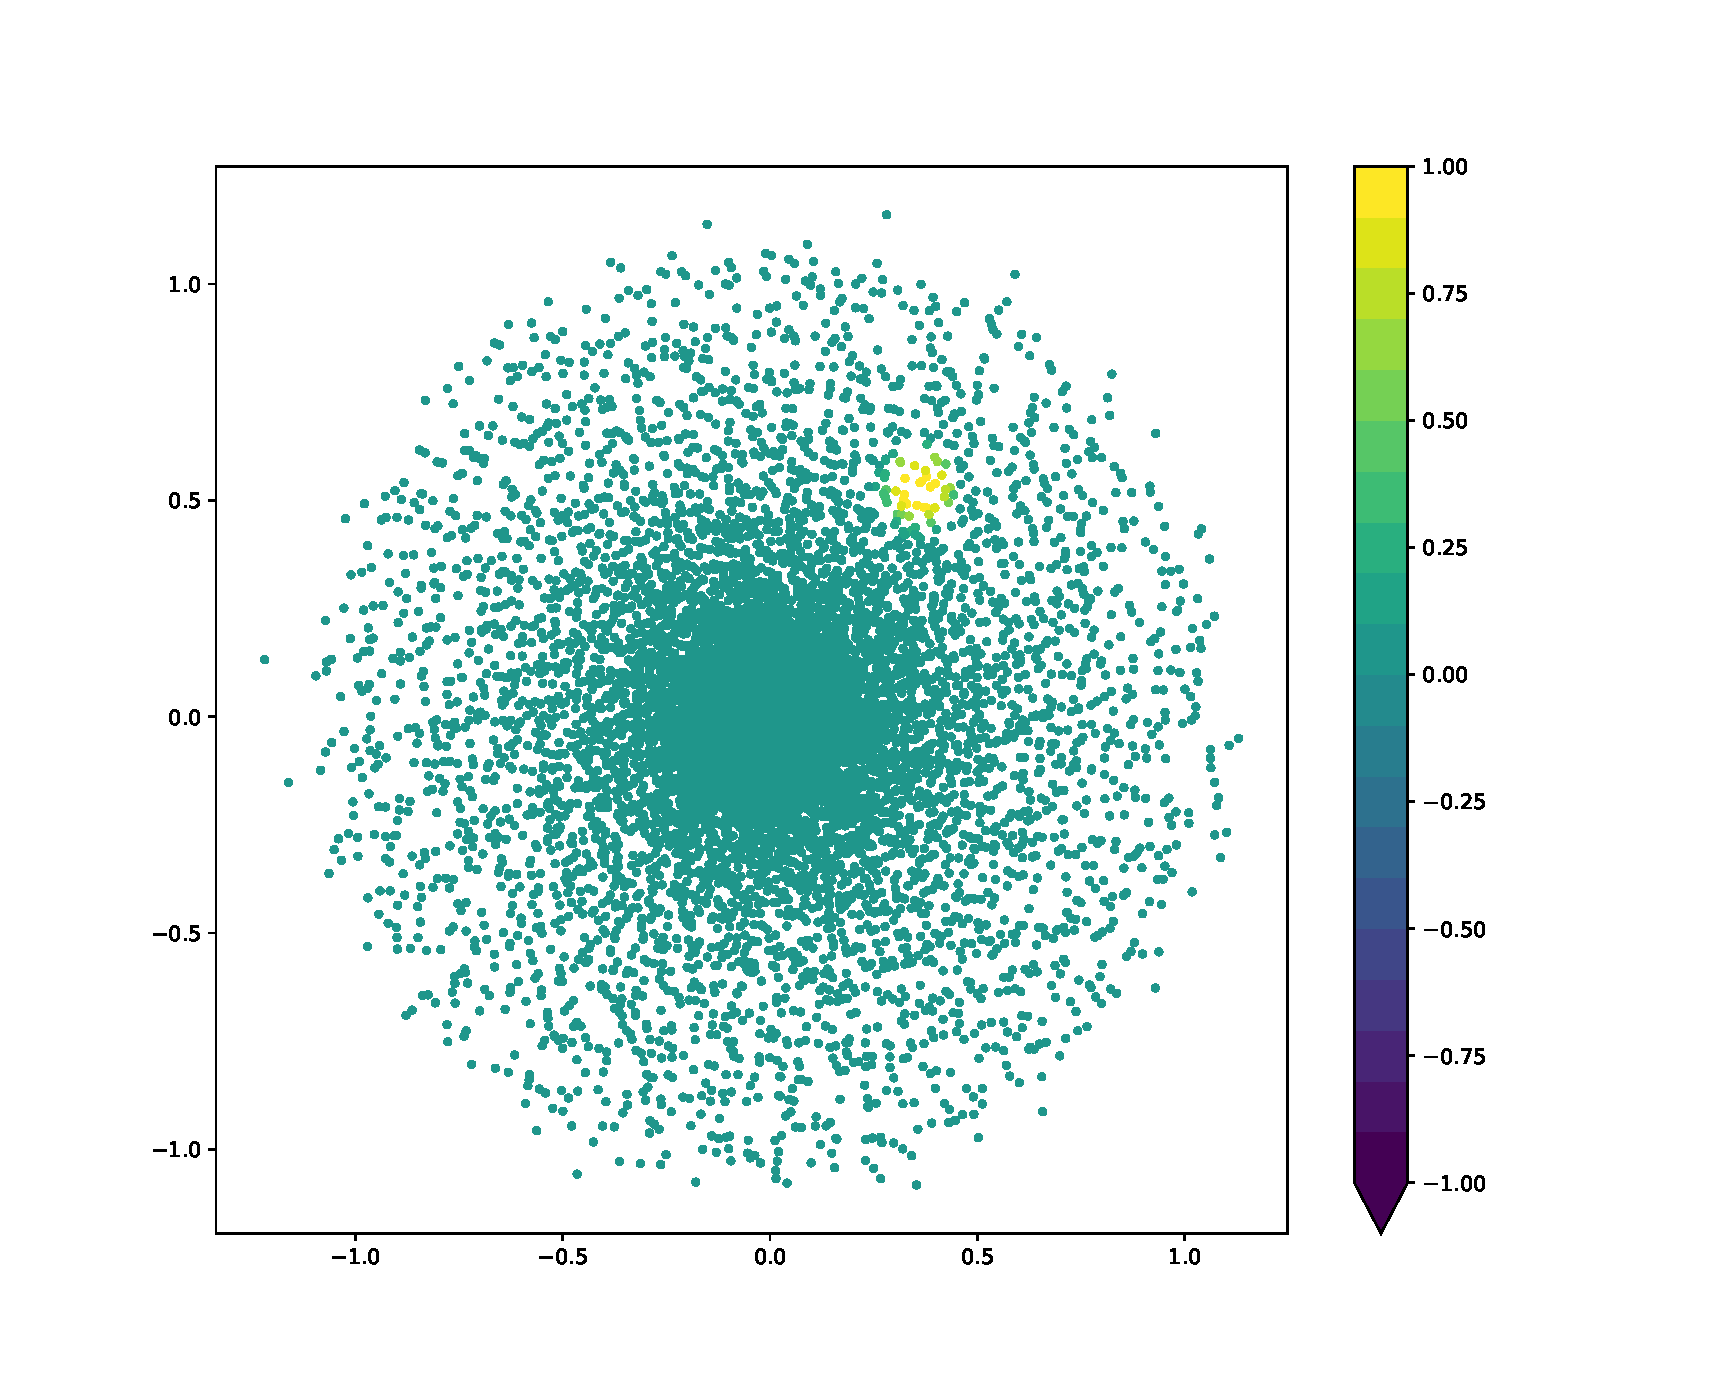
\includegraphics[width=\textwidth]{figures/onv_normal_cur.pdf}
        \caption{Current ONV}
        \label{fig:onv_cur}
    \end{subfigure}
    \hfill
    \begin{subfigure}[b]{0.45\textwidth}
        \centering
        % \includesvg{onv_delta.svg}
        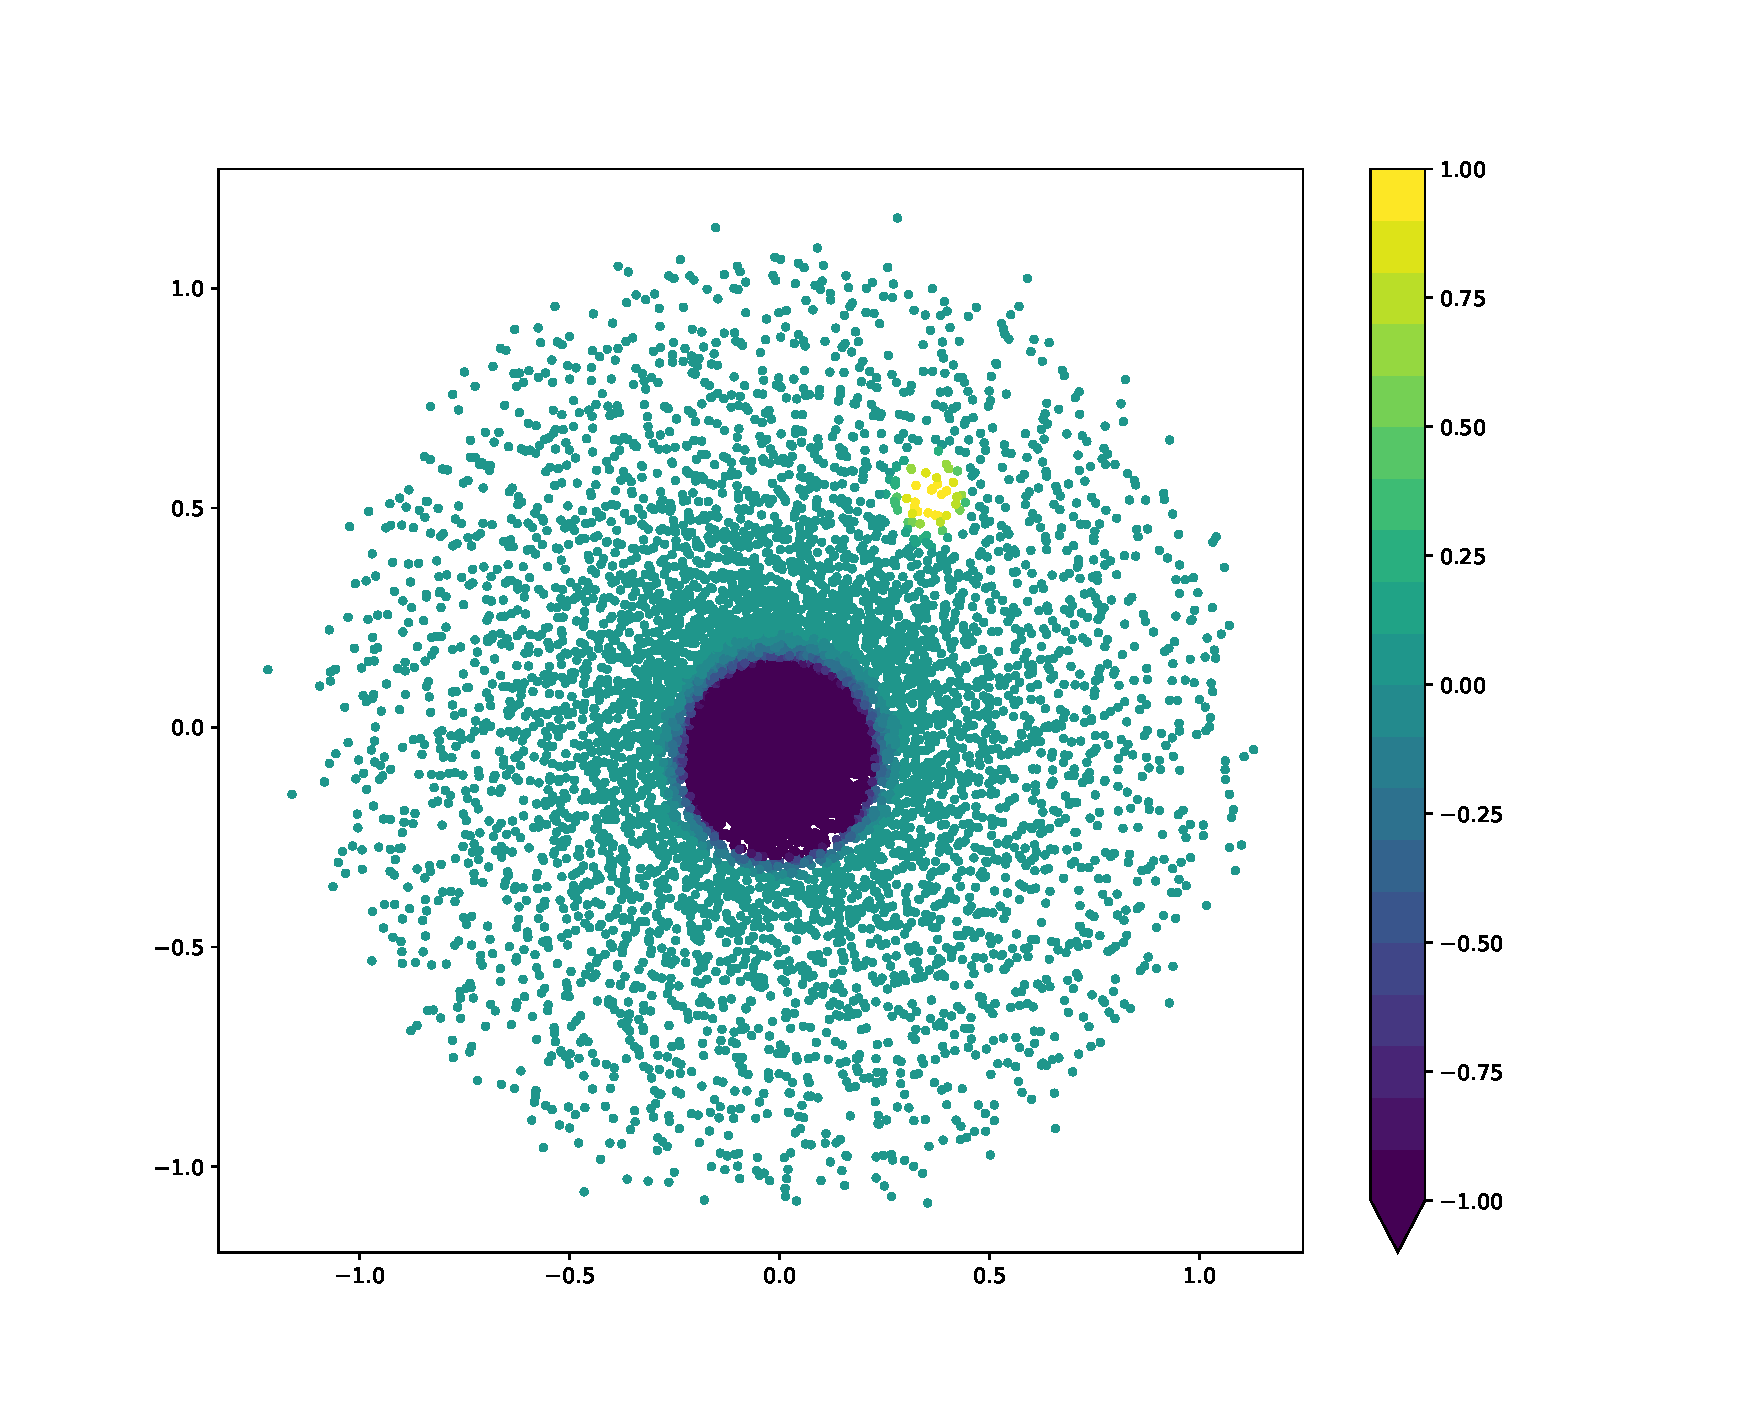
\includegraphics[width=\textwidth]{figures/onv_delta.pdf}
        \caption{Delta ONV}
        \label{fig:onv_delta}
    \end{subfigure}
    \caption{We map the ONV values to the log-polar distribution. The target has moved from (a) to (b). (c) shows the corresponding delta ONV, where we can see the values darkened where the target was in (a) and got brighter at the target's location in (b).}
    \label{fig:three ONVs}
\end{figure}

%%%%%%%%%%%%%%%%%%%%%%%%%%%%%%%%%%%%%%%%%%%%%%%%%%%%%%%%%%%%%%%%%%%%%%

% do I need this higher level organization?
\subsection{Spiking Inputs}

In this section we review the two most popular encoding methods, rate and latency. It is believed that each method is used in different parts of the brain and even the visual cortex. One theory is that the retina uses rate encoding but more downstream neurons use latency encoding. We empirically found that rate encoding performed better than latency encoding on our object tracking task.

%%%%%%%%%%%%%%%%%%%%%%%%%%%%%%%%%%%%%%%%%%%%%%%%%%%%%%%%%%%%%%%%%%%%%%

\subsubsection{Rate Encoding}

Rate encoding attempts to encode a neuron's firing frequency. Each input value to the encoder is between 0 and 1, representing the probability that the neuron will spike at a given timestep. Then, at each timestep, we run a Bernoulli trial to see if the neuron will spike with the given probability.

For example, if our photoreceptor value was 0, the neuron would never spike. On the other hand, a value of 1 would create spikes at each timestep. A value of 0.5 would result in about half of the timesteps containing a spike. We show these examples over 20 timesteps in figure \ref{fig:rate_encode_3plots}.

\begin{figure}[h]
    \centering
    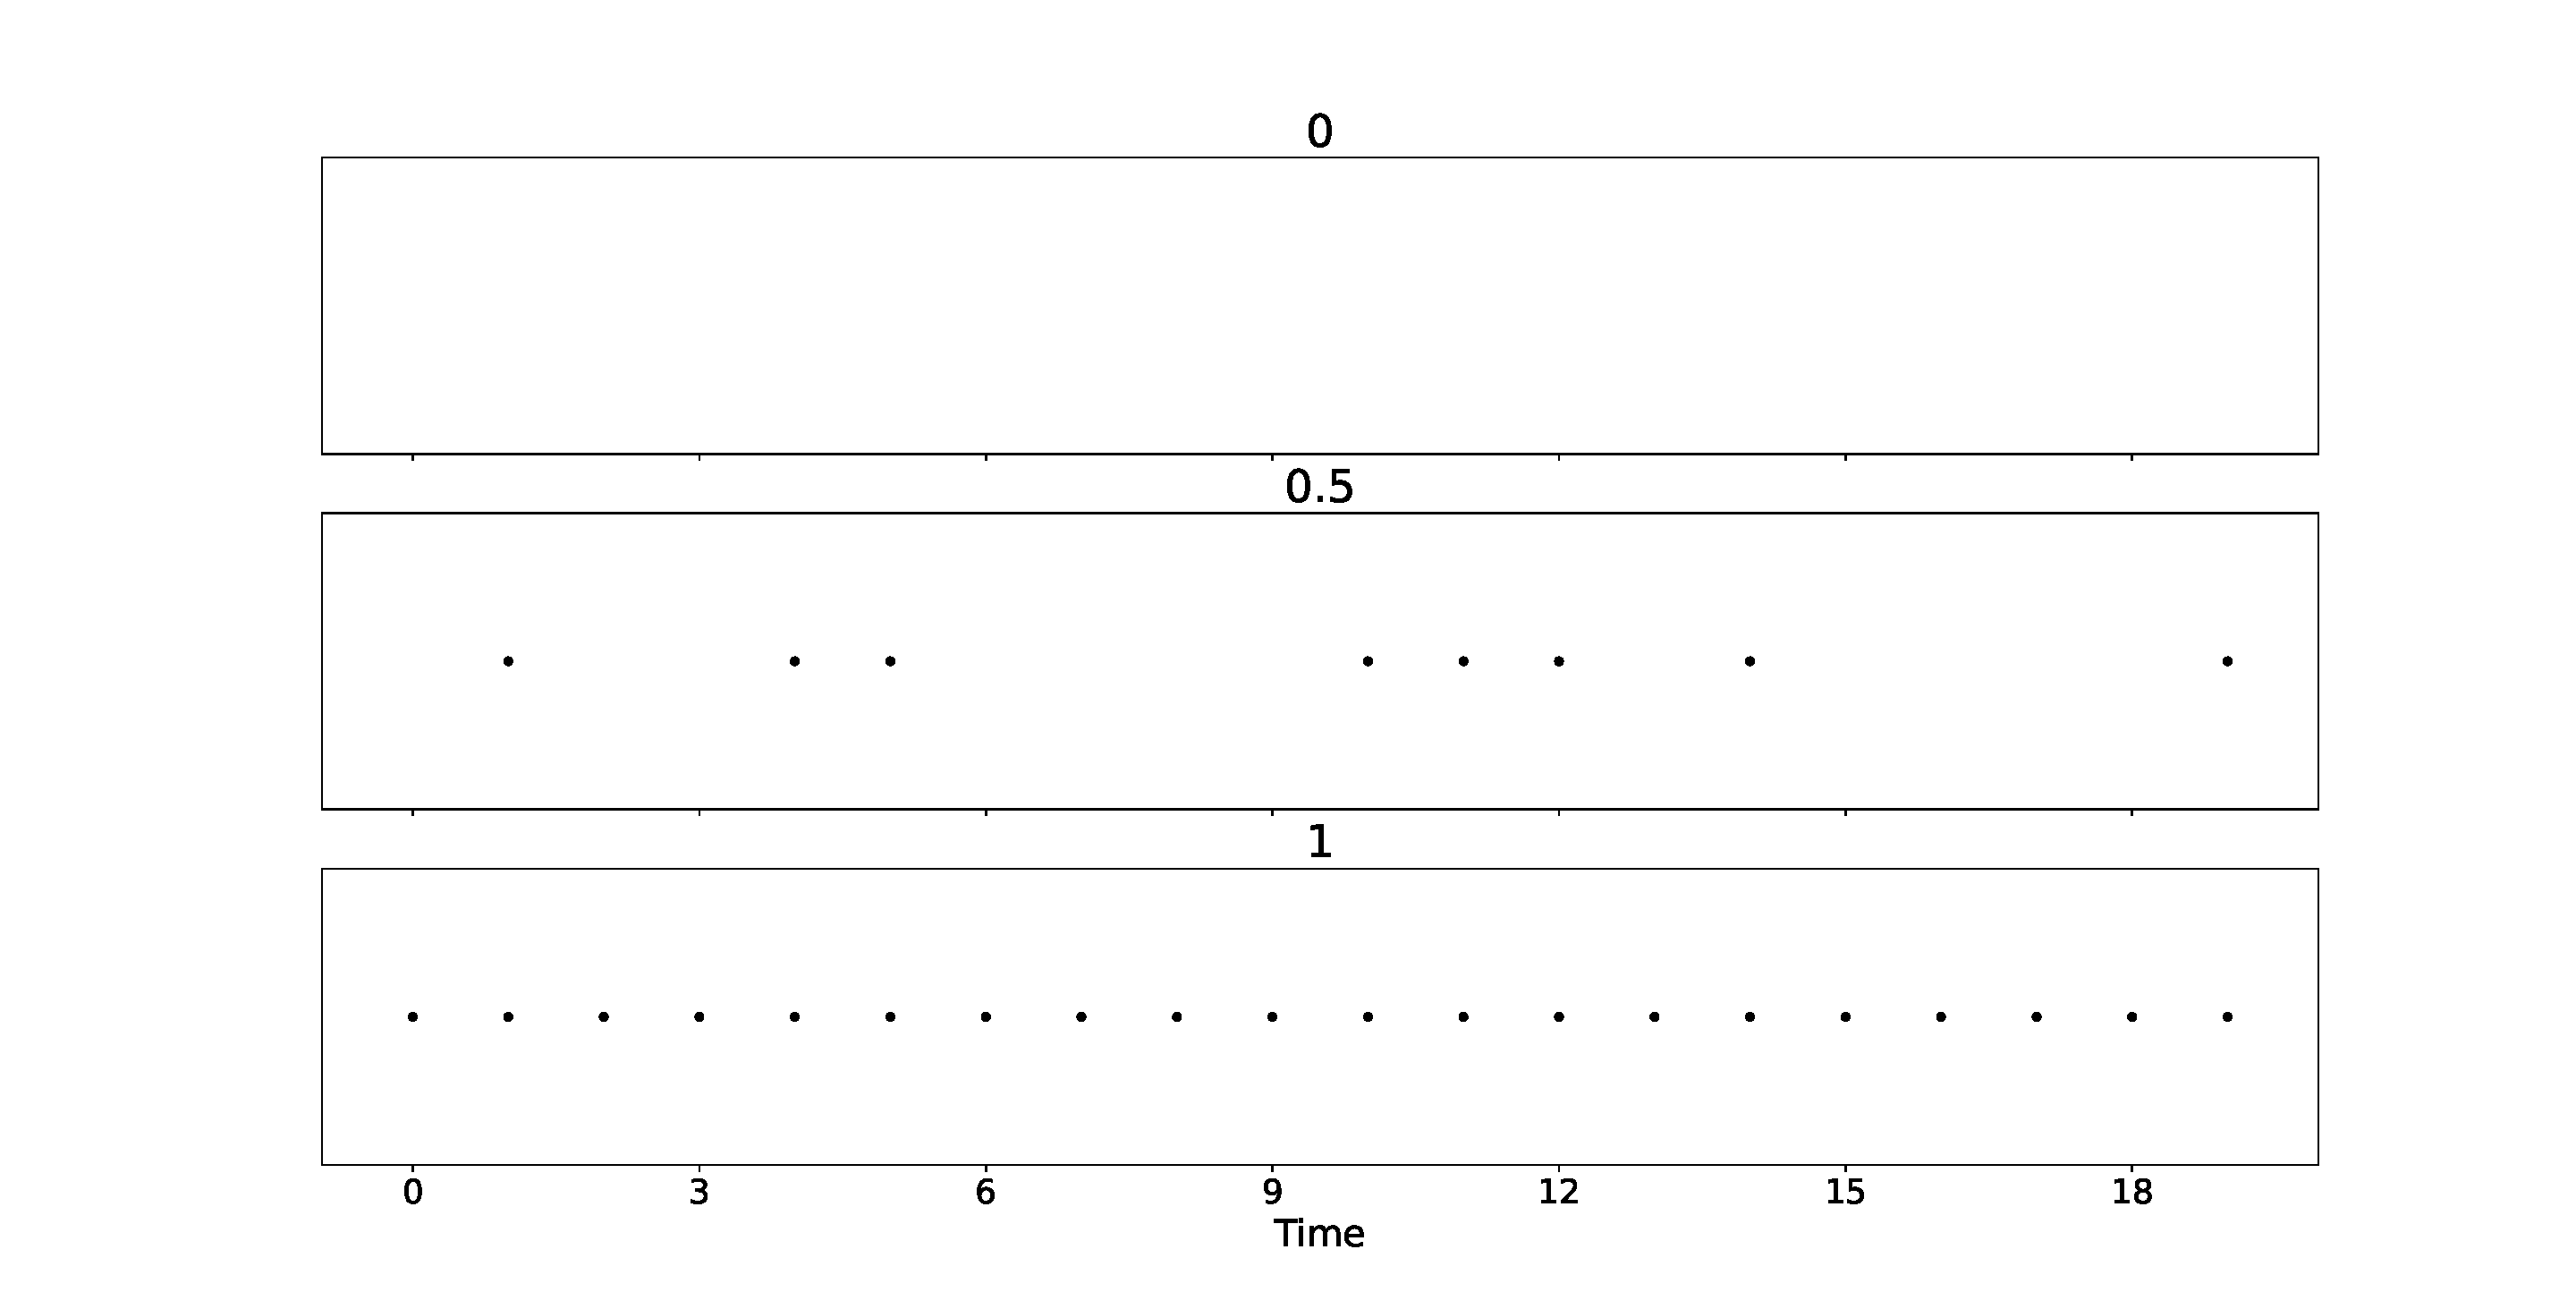
\includegraphics[width=0.6\textwidth]{figures/neuron_3_rate.pdf}
    \caption{Demonstration of rate encoding. From top to bottom we encode data with values of 0, 0.5, and 1.}
    \label{fig:rate_encode_3plots}
\end{figure}

\begin{figure}[h]
    \centering
    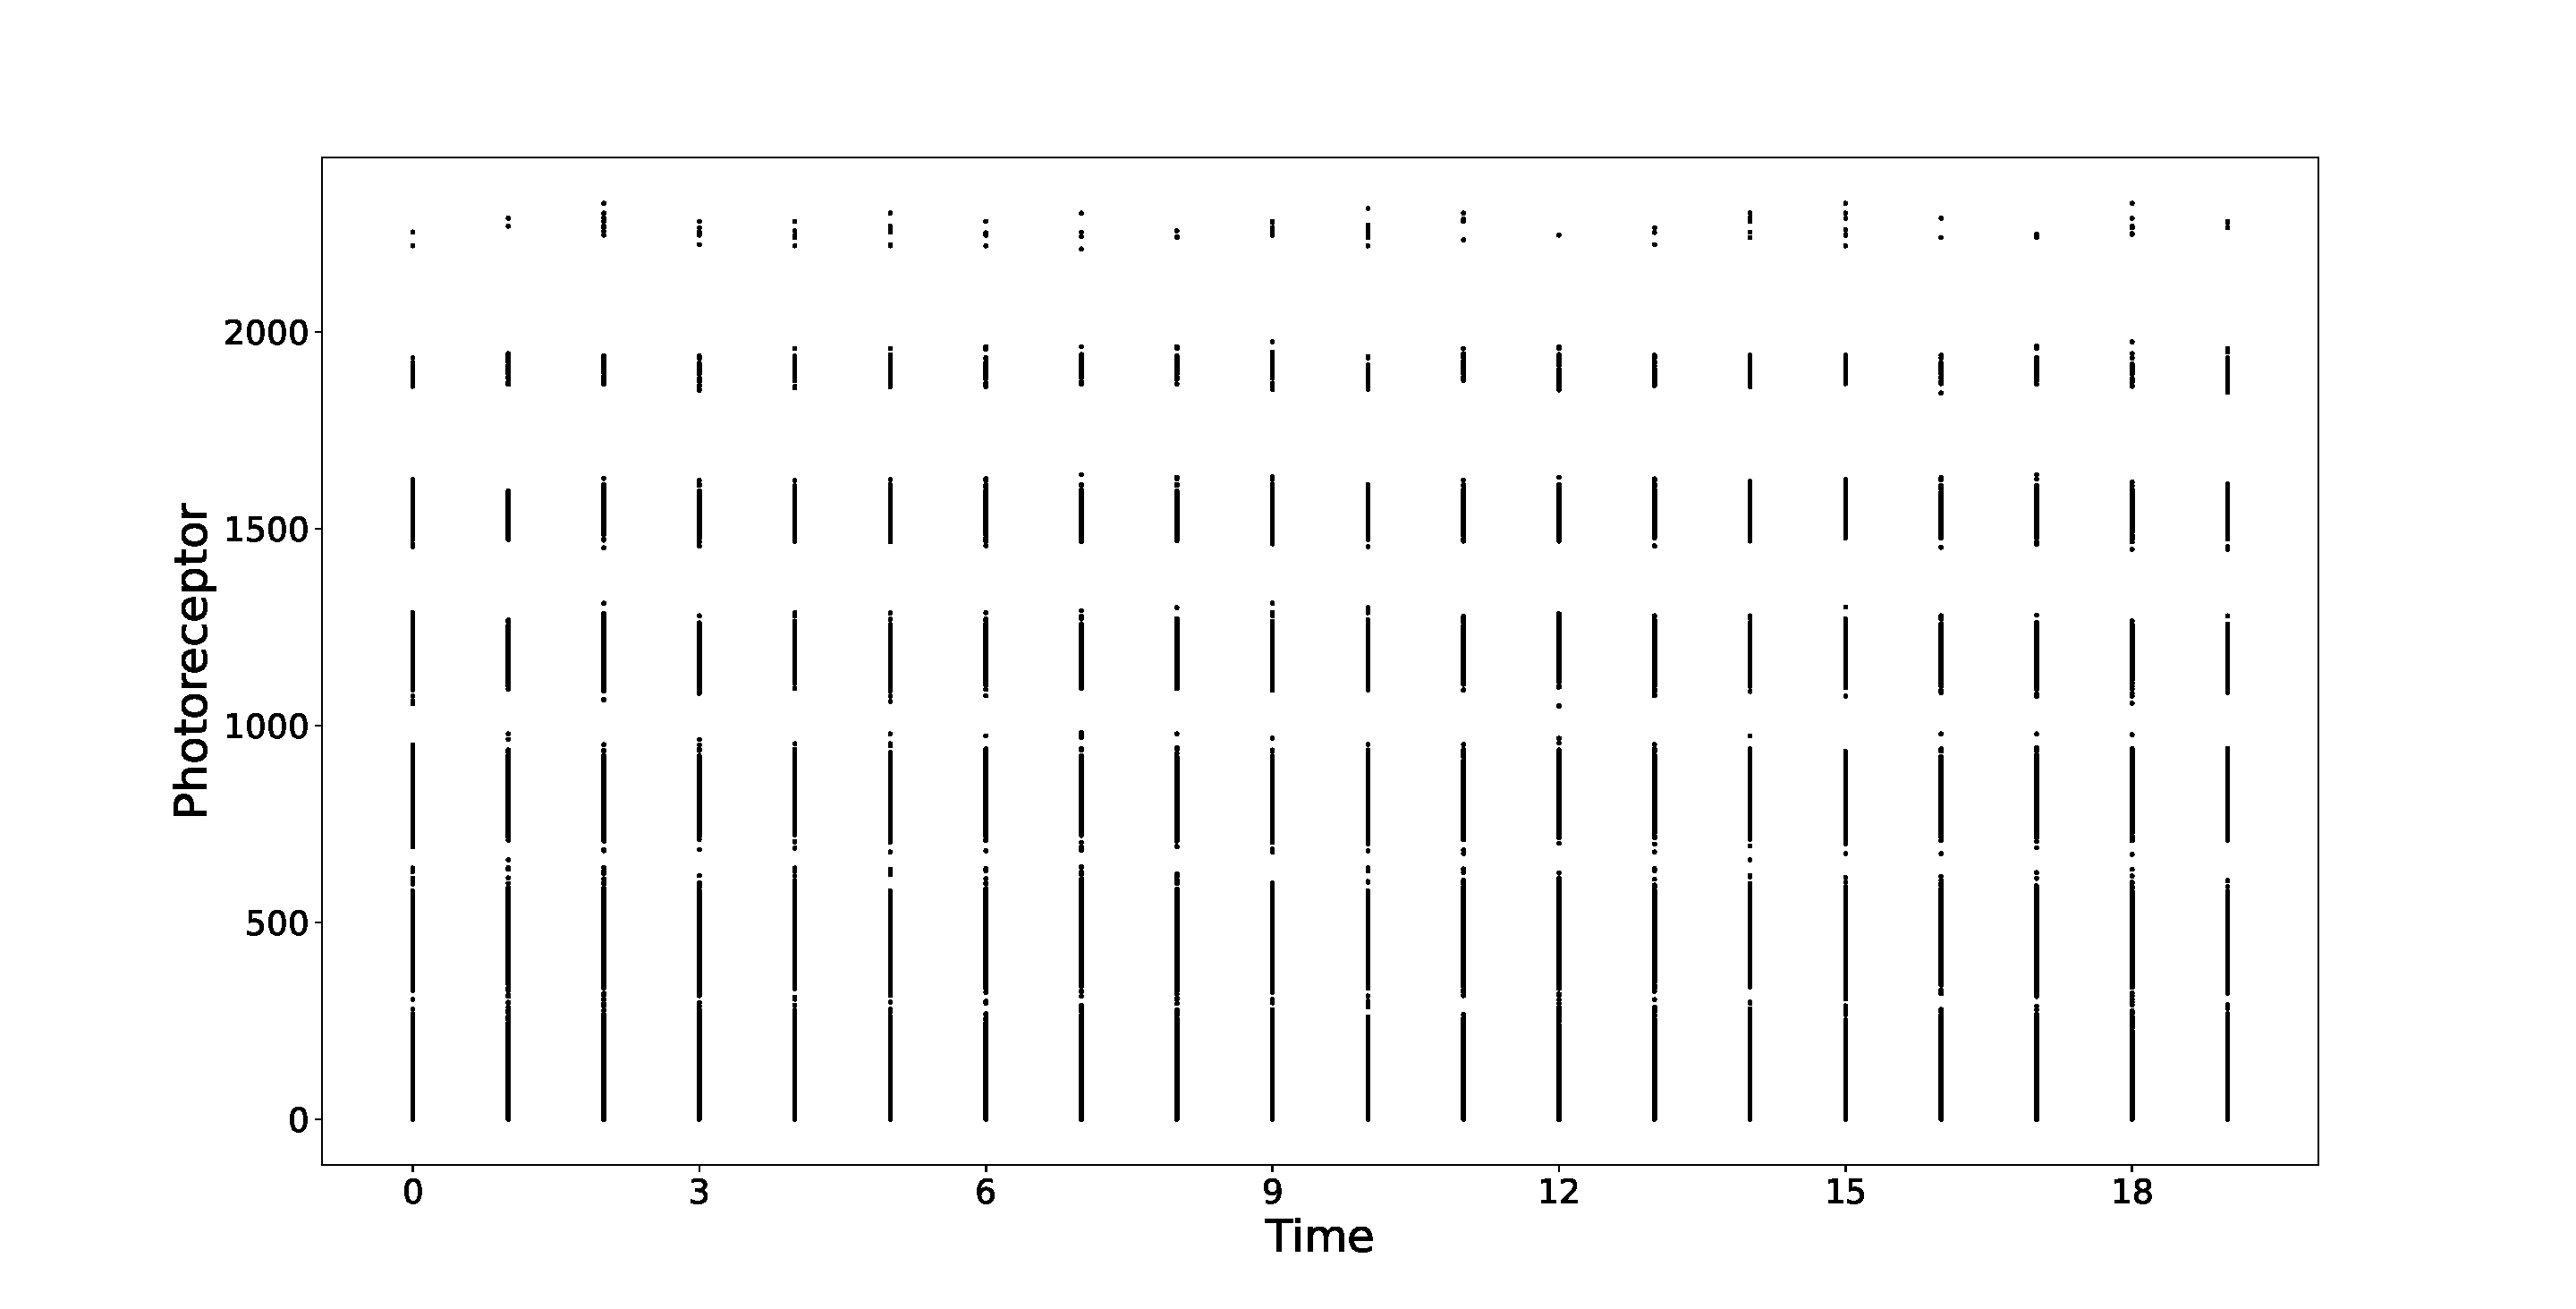
\includegraphics[width=0.7\textwidth]{figures/onv_rate_prev.pdf}
    \caption{Rate encoding of the ONV from \ref{fig:onv_prev}. We look at a subset of the 14,400 neurons. Only the photoreceptors with non-zero values are spiking, and we can see different spike rates corresponding to different light intensities. }
    \label{fig:onv_encode_rate}
\end{figure}

Each of our RGB color channels are already in the range of 0 to 1, so they can directly be rate encoded. We present a subset of the input spikes that result from rate encoding the ONV from figure \ref{fig:onv_prev}. We can see a few different firing rates in the figure, with excited neurons firing at every timestep and other neurons not firing at all.

With the delta ONV, however, we have values in the range of -1 to 1. This is a problem because we cannot have a negative probability assigned to whether or not an input neuron will spike. The solution is to take the absolute value of the probability, and if a spike is generated, it will carry a value of -1 instead of 1. This means that neurons in the next layer will decrease their internal voltage if they receive a spike with value -1. Figure \ref{fig:negative_spike_example} shows what happens when a neuron receives negative spikes.

\begin{figure}[h]
    \centering
    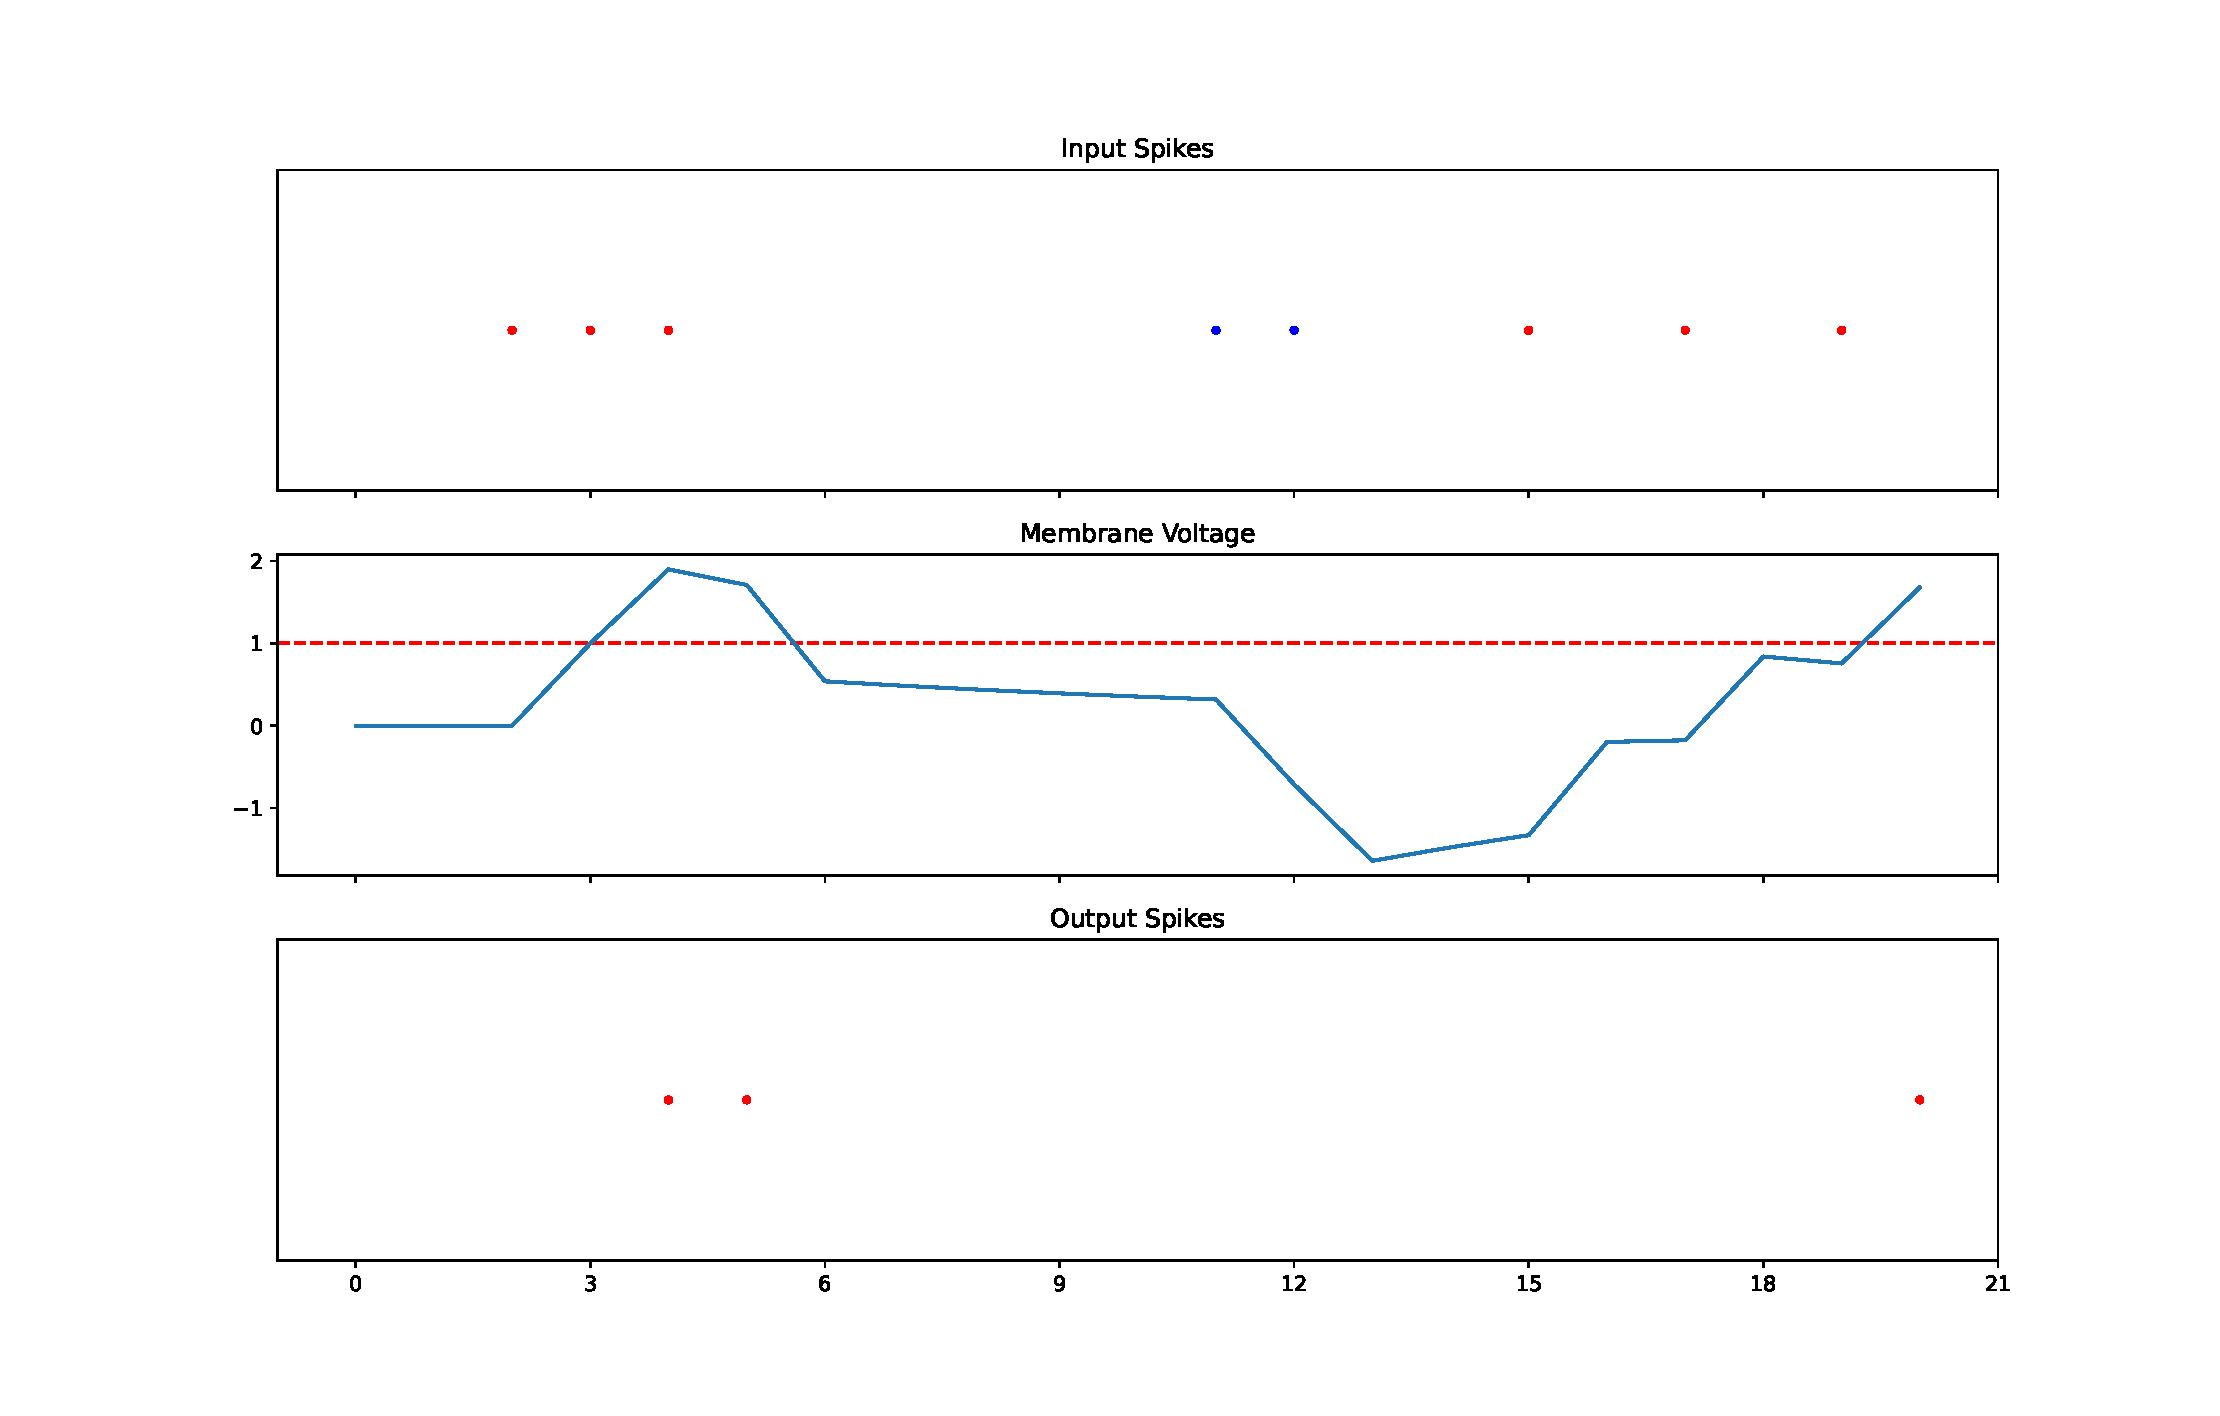
\includegraphics[width=0.8\textwidth]{figures/negative_spike_example.pdf}
    \caption{Example with negative spikes input to the neuron. Positive spikes are shown in red, negative in blue.}
    \label{fig:negative_spike_example}
\end{figure}

The inputs to the rate encoder can also be scaled up before being turned into spikes. This is referred to as the gain, which we treat as a hyperparameter. For example, given gain $g$ and input $x$, our new input becomes $g*x$. Values above 1 are clipped to 1.

Larger gain values seemed to create a smoother decrease in loss and better training performance. Intuitively this makes sense because this creates more spikes in the input layer and gives downstream neurons more opportunities to fire. However, larger gain values also led to higher validation loss and resulted in models that could not track the target during inference. We limit the amount of gain to 2, meaning that photoreceptors with values 0.5 and above spiked at every timestep.

% loss graph of tuning gain?

%%%%%%%%%%%%%%%%%%%%%%%%%%%%%%%%%%%%%%%%%%%%%%%%%%%%%%%%%%%%%%%%%%%%%%

\subsubsection{Latency Encoding}

Latency encoding, on the other hand, focuses on the timing of spikes rather than the spike rate. Each neuron is allowed to fire once in the simulated time interval; neurons with a higher probability of firing emit their spike earlier than neurons with lower probabilities of spiking. This encoding method results in sparser inputs to the SNN when compared to rate encoding and as a result also makes it difficult for the model to converge.

Figure \ref{fig:onv_encode_latency} contains spikes that result from latency encoding the onv from figure \ref{fig:onv_prev}. In the figure we see that very excited neurons fire at the first timestep and partially excited neurons fire sometime afterwards. The spikes at the last timestep represent inputs of 0.

\begin{figure}[h]
    \centering
    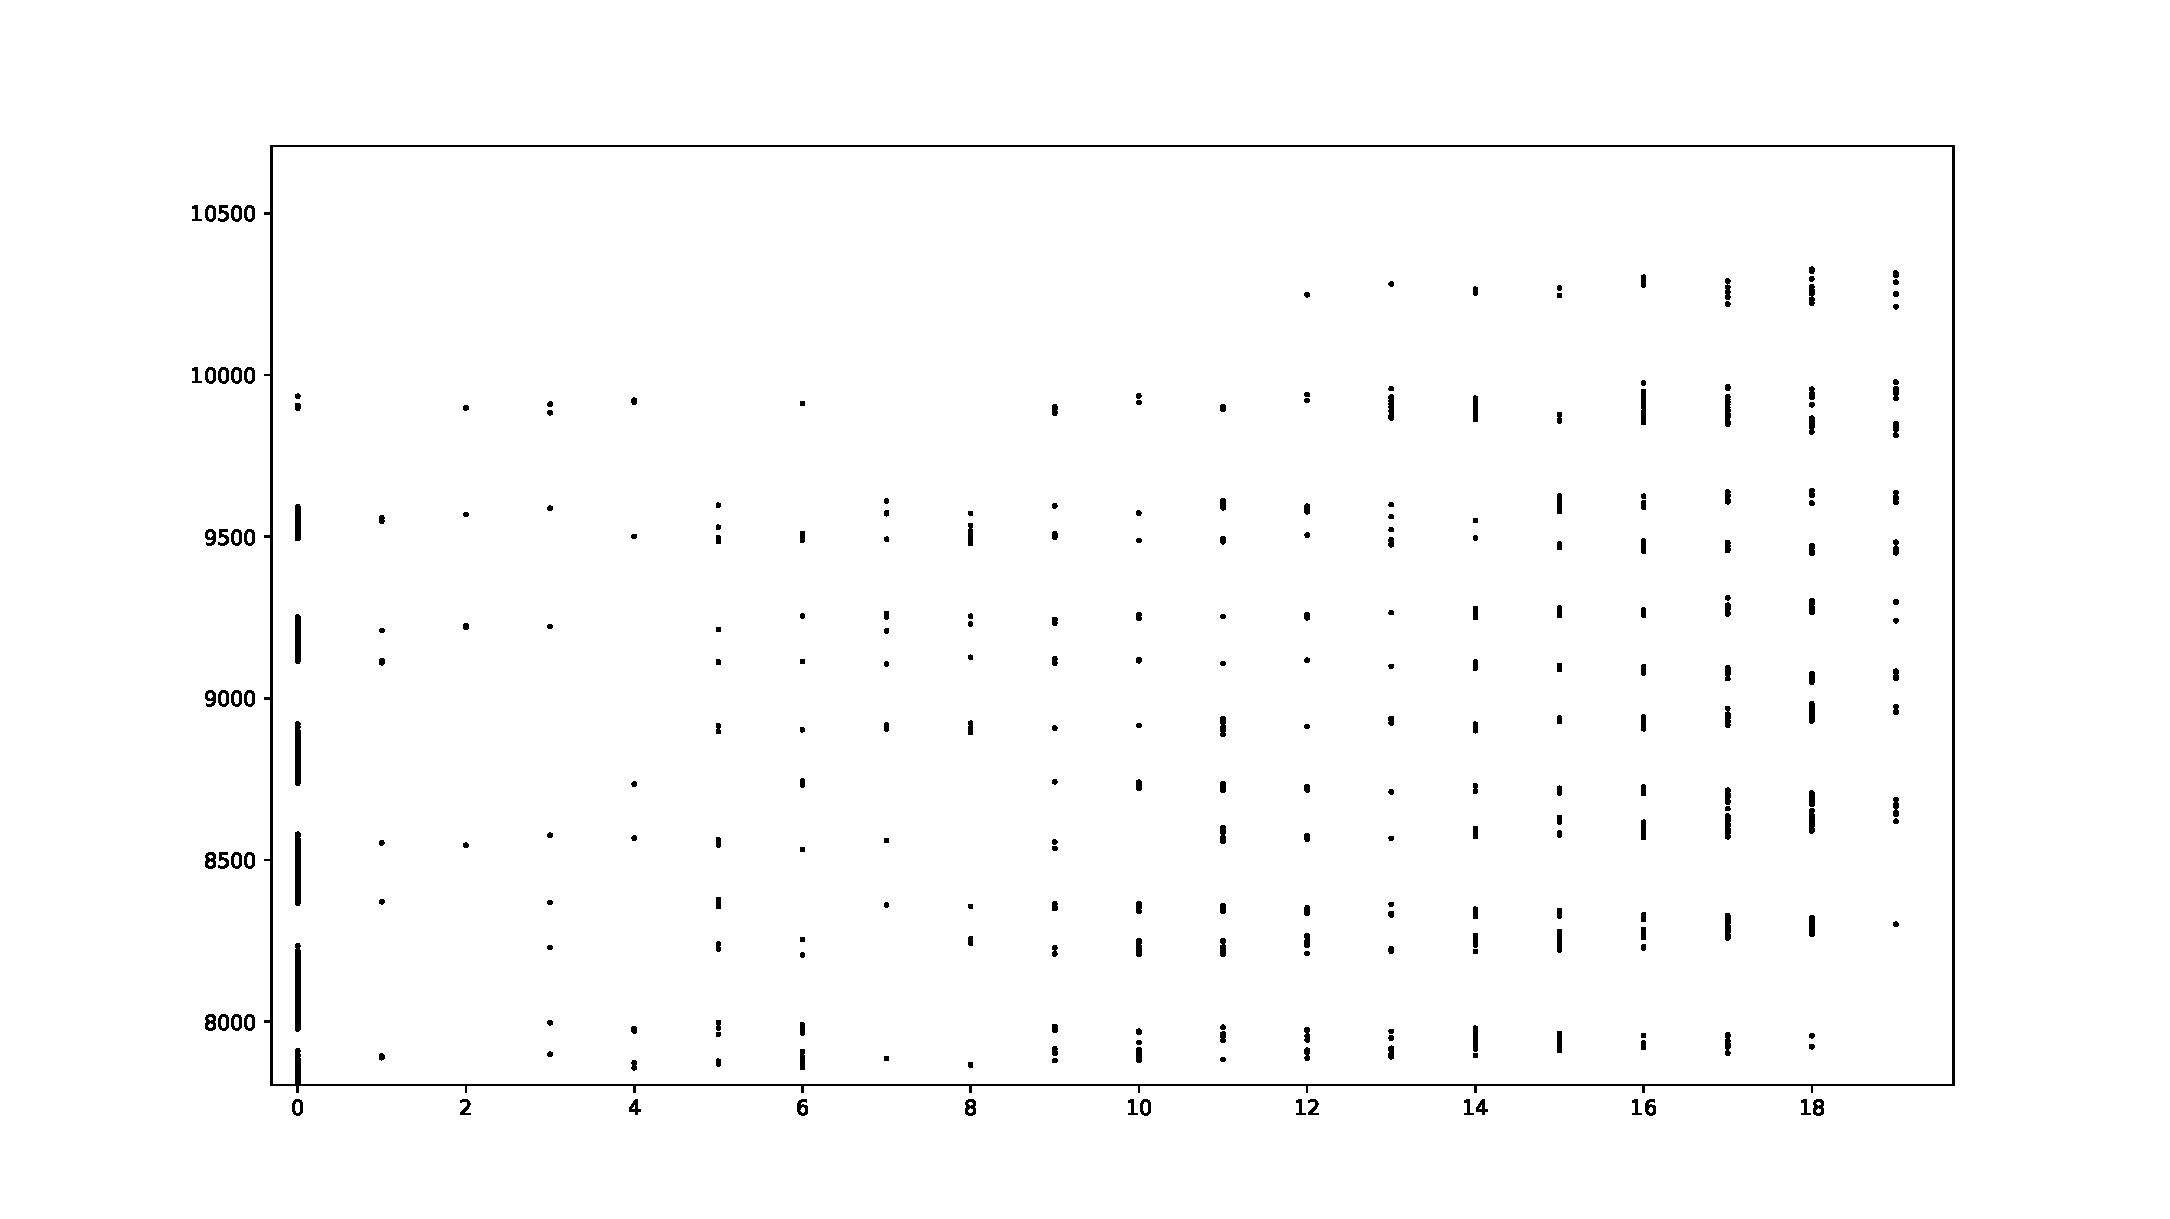
\includegraphics[width=0.6\textwidth]{figures/onv_latency_prev.pdf}
    \caption{Latency encoding of the ONV from \ref{fig:onv_cur}.  We look at a subset of the 14,400 neurons. The values are normalized to fit within a 20 timestep range. The values to the left have the highest spike probability and the values to the right have low probabilities.}
    \label{fig:onv_encode_latency}
\end{figure}

%%%%%%%%%%%%%%%%%%%%%%%%%%%%%%%%%%%%%%%%%%%%%%%%%%%%%%%%%%%%%%%%%%%%%%

\end{document}